\section{Benchmark 9: Vorticity-Induced Gravity vs General Relativity}

In the Vortex Æther Model (VAM), gravitational attraction arises not from spacetime curvature, but from swirl-induced pressure gradients within a compressible, incompressible superfluid æther. The gravitational potential is thus reconstructed from vorticity fields.

\subsection{VAM Swirl Potential}

Assuming a radially symmetric vortex field with angular velocity profile:

\begin{equation}
\omega(r) = \frac{C_e}{r_c} e^{-r/r_c}
\end{equation}

the corresponding swirl-induced gravitational potential is given by:

\begin{equation}
\Phi_{\text{VAM}}(r) = \frac{C_e^2}{2 F_{\text{max}}} \, \omega(r) \cdot r = \frac{C_e^3}{2 F_{\text{max}} r_c} \, r \, e^{-r/r_c}
\end{equation}

This potential:
\begin{itemize}
    \item Remains finite at \( r \to 0 \),
    \item Peaks near \( r \sim r_c \),
    \item Decays exponentially for \( r \gg r_c \), ensuring localized gravitational wells.
\end{itemize}

\subsection{Comparison with General Relativity}

The Newtonian limit of General Relativity yields the Schwarzschild gravitational potential:

\begin{equation}
\Phi_{\text{GR}}(r) = -\frac{G M}{r}
\end{equation}

which diverges at \( r \to 0 \) and falls off as a power law at large \( r \), enabling long-range interactions.

\begin{figure}[H]
    \centering
    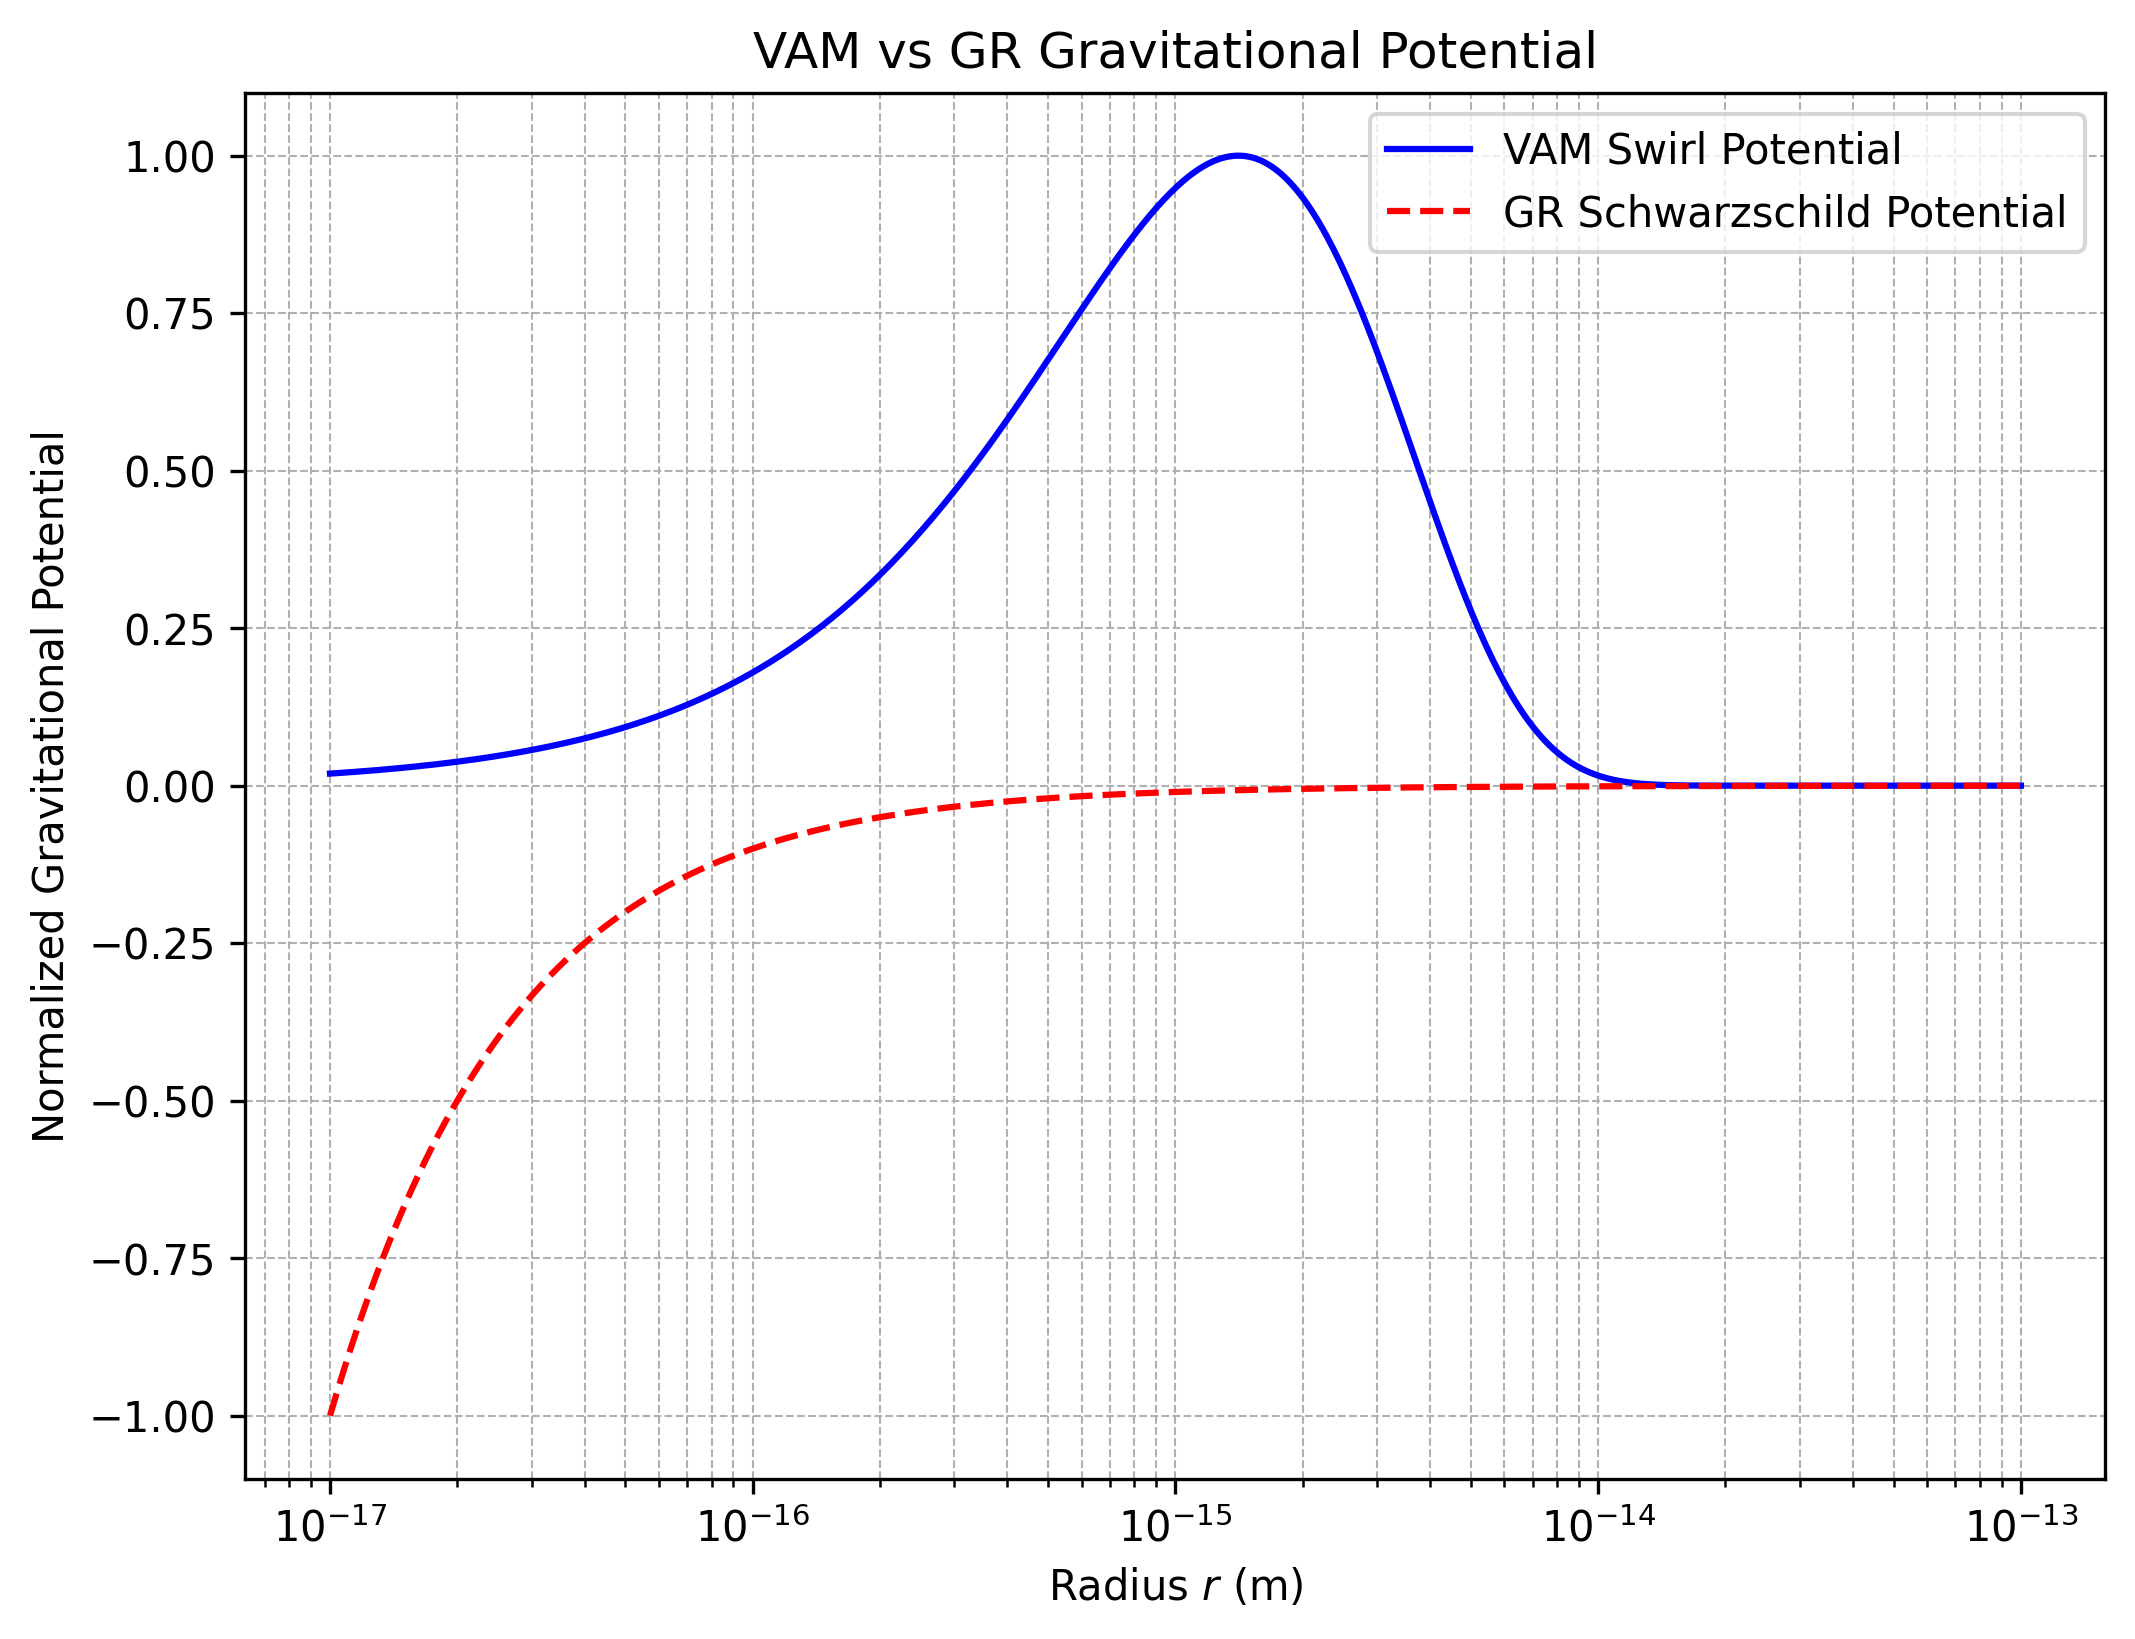
\includegraphics[width=0.65\textwidth]{vam_vs_gr_potential_plot.png}
    \caption{Comparison between the VAM swirl potential (solid) and the GR Schwarzschild potential (dashed). The VAM potential saturates at small \( r \), eliminating divergences and singularities.}
\end{figure}

\subsection{Physical Consequences}

\begin{itemize}
    \item VAM predicts a \textbf{finite gravitational self-potential} for compact bodies, avoiding singularities.
    \item The decay length is controlled by \( r_c \), linking gravity's range to vortex core radius.
    \item At galactic scales, VAM predicts effectively short-range gravitational potentials unless coupled to global swirl structures (e.g., vortex chains, filaments).
\end{itemize}

\subsection{Conclusion}

The swirl potential derived from structured vorticity in VAM reproduces gravitational-like behavior at intermediate scales, resolves divergence at small \( r \), and introduces natural cutoff behavior at large distances. This forms a coherent alternative to the Schwarzschild solution, with clear physical origin in vortex structure.
